\Problem
{\lr{ARFCN} چیست؟}
{
\lr{Absolute Radio Frequency Channel Number}
یا به اختصار
\lr{ARFCN}
کدی است که یک جفت حامل رادیویی فیزیکی را مشخص می‌کند.

با توجه به اعشاری بودن مقادیر فرکانس کار کردن با اعداد آن سخت است.
نکته دیگر این است که فرکانس‌ها در یک بازه تعریف می‌شوند که اعداد آن زیاد است و ما باید فرکانس مرکزی آن را در نظر بگیریم.
این مشکلات باعث می‌شود به هر حامل یک شماره اختصاص دهیم که منحصر به فرد است. از این معیار می‌توان برای محاسبه دقیق فرکانس استفاده کنیم.

مقادیر آن در جدول زیر برای چند کانال آورده شده است.
\begin{figure}[H]
    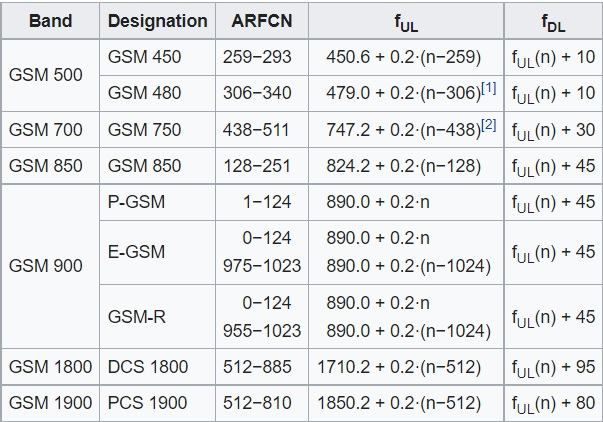
\includegraphics[width=10cm]{Images/ARFCN.jpg}
    \centering
    \caption{\lr{ARFCN}}
\end{figure}

نحوه محاسبه آن به صورت زیر است:
\begin{equation*}
    n = \frac{f - f_b - f_o}{f_c}
\end{equation*}

\begin{equation*}
    f = (f_c \times n) + f_b + f_o
\end{equation*}

\lr{n}
نشان دهنده عدد
\lr{ARFCN}
است.

\lr{$f_b$}
فرکانس شروع باند است.

\lr{$f_o$}
فرکانس ست شدن است.

\lr{$f_c$}
فرکانس فاصله کانال است.
}
